\documentclass[1p]{elsarticle_modified}
%\bibliographystyle{elsarticle-num}

%\usepackage[colorlinks]{hyperref}
%\usepackage{abbrmath_seonhwa} %\Abb, \Ascr, \Acal ,\Abf, \Afrak
\usepackage{amsfonts}
\usepackage{amssymb}
\usepackage{amsmath}
\usepackage{amsthm}
\usepackage{scalefnt}
\usepackage{amsbsy}
\usepackage{kotex}
\usepackage{caption}
\usepackage{subfig}
\usepackage{color}
\usepackage{graphicx}
\usepackage{xcolor} %% white, black, red, green, blue, cyan, magenta, yellow
\usepackage{float}
\usepackage{setspace}
\usepackage{hyperref}

\usepackage{tikz}
\usetikzlibrary{arrows}

\usepackage{multirow}
\usepackage{array} % fixed length table
\usepackage{hhline}

%%%%%%%%%%%%%%%%%%%%%
\makeatletter
\renewcommand*\env@matrix[1][\arraystretch]{%
	\edef\arraystretch{#1}%
	\hskip -\arraycolsep
	\let\@ifnextchar\new@ifnextchar
	\array{*\c@MaxMatrixCols c}}
\makeatother %https://tex.stackexchange.com/questions/14071/how-can-i-increase-the-line-spacing-in-a-matrix
%%%%%%%%%%%%%%%

\usepackage[normalem]{ulem}

\newcommand{\msout}[1]{\ifmmode\text{\sout{\ensuremath{#1}}}\else\sout{#1}\fi}
%SOURCE: \msout is \stkout macro in https://tex.stackexchange.com/questions/20609/strikeout-in-math-mode

\newcommand{\cancel}[1]{
	\ifmmode
	{\color{red}\msout{#1}}
	\else
	{\color{red}\sout{#1}}
	\fi
}

\newcommand{\add}[1]{
	{\color{blue}\uwave{#1}}
}

\newcommand{\replace}[2]{
	\ifmmode
	{\color{red}\msout{#1}}{\color{blue}\uwave{#2}}
	\else
	{\color{red}\sout{#1}}{\color{blue}\uwave{#2}}
	\fi
}

\newcommand{\Sol}{\mathcal{S}} %segment
\newcommand{\D}{D} %diagram
\newcommand{\A}{\mathcal{A}} %arc


%%%%%%%%%%%%%%%%%%%%%%%%%%%%%5 test

\def\sl{\operatorname{\textup{SL}}(2,\Cbb)}
\def\psl{\operatorname{\textup{PSL}}(2,\Cbb)}
\def\quan{\mkern 1mu \triangleright \mkern 1mu}

\theoremstyle{definition}
\newtheorem{thm}{Theorem}[section]
\newtheorem{prop}[thm]{Proposition}
\newtheorem{lem}[thm]{Lemma}
\newtheorem{ques}[thm]{Question}
\newtheorem{cor}[thm]{Corollary}
\newtheorem{defn}[thm]{Definition}
\newtheorem{exam}[thm]{Example}
\newtheorem{rmk}[thm]{Remark}
\newtheorem{alg}[thm]{Algorithm}

\newcommand{\I}{\sqrt{-1}}
\begin{document}

%\begin{frontmatter}
%
%\title{Boundary parabolic representations of knots up to 8 crossings}
%
%%% Group authors per affiliation:
%\author{Yunhi Cho} 
%\address{Department of Mathematics, University of Seoul, Seoul, Korea}
%\ead{yhcho@uos.ac.kr}
%
%
%\author{Seonhwa Kim} %\fnref{s_kim}}
%\address{Center for Geometry and Physics, Institute for Basic Science, Pohang, 37673, Korea}
%\ead{ryeona17@ibs.re.kr}
%
%\author{Hyuk Kim}
%\address{Department of Mathematical Sciences, Seoul National University, Seoul 08826, Korea}
%\ead{hyukkim@snu.ac.kr}
%
%\author{Seokbeom Yoon}
%\address{Department of Mathematical Sciences, Seoul National University, Seoul, 08826,  Korea}
%\ead{sbyoon15@snu.ac.kr}
%
%\begin{abstract}
%We find all boundary parabolic representation of knots up to 8 crossings.
%
%\end{abstract}
%\begin{keyword}
%    \MSC[2010] 57M25 
%\end{keyword}
%
%\end{frontmatter}

%\linenumbers
%\tableofcontents
%
\newcommand\colored[1]{\textcolor{white}{\rule[-0.35ex]{0.8em}{1.4ex}}\kern-0.8em\color{red} #1}%
%\newcommand\colored[1]{\textcolor{white}{ #1}\kern-2.17ex	\textcolor{white}{ #1}\kern-1.81ex	\textcolor{white}{ #1}\kern-2.15ex\color{red}#1	}

{\Large $\underline{12n_{0104}~(K12n_{0104})}$}

\setlength{\tabcolsep}{10pt}
\renewcommand{\arraystretch}{1.6}
\vspace{1cm}\begin{tabular}{m{100pt}>{\centering\arraybackslash}m{274pt}}
\multirow{5}{120pt}{
	\centering
	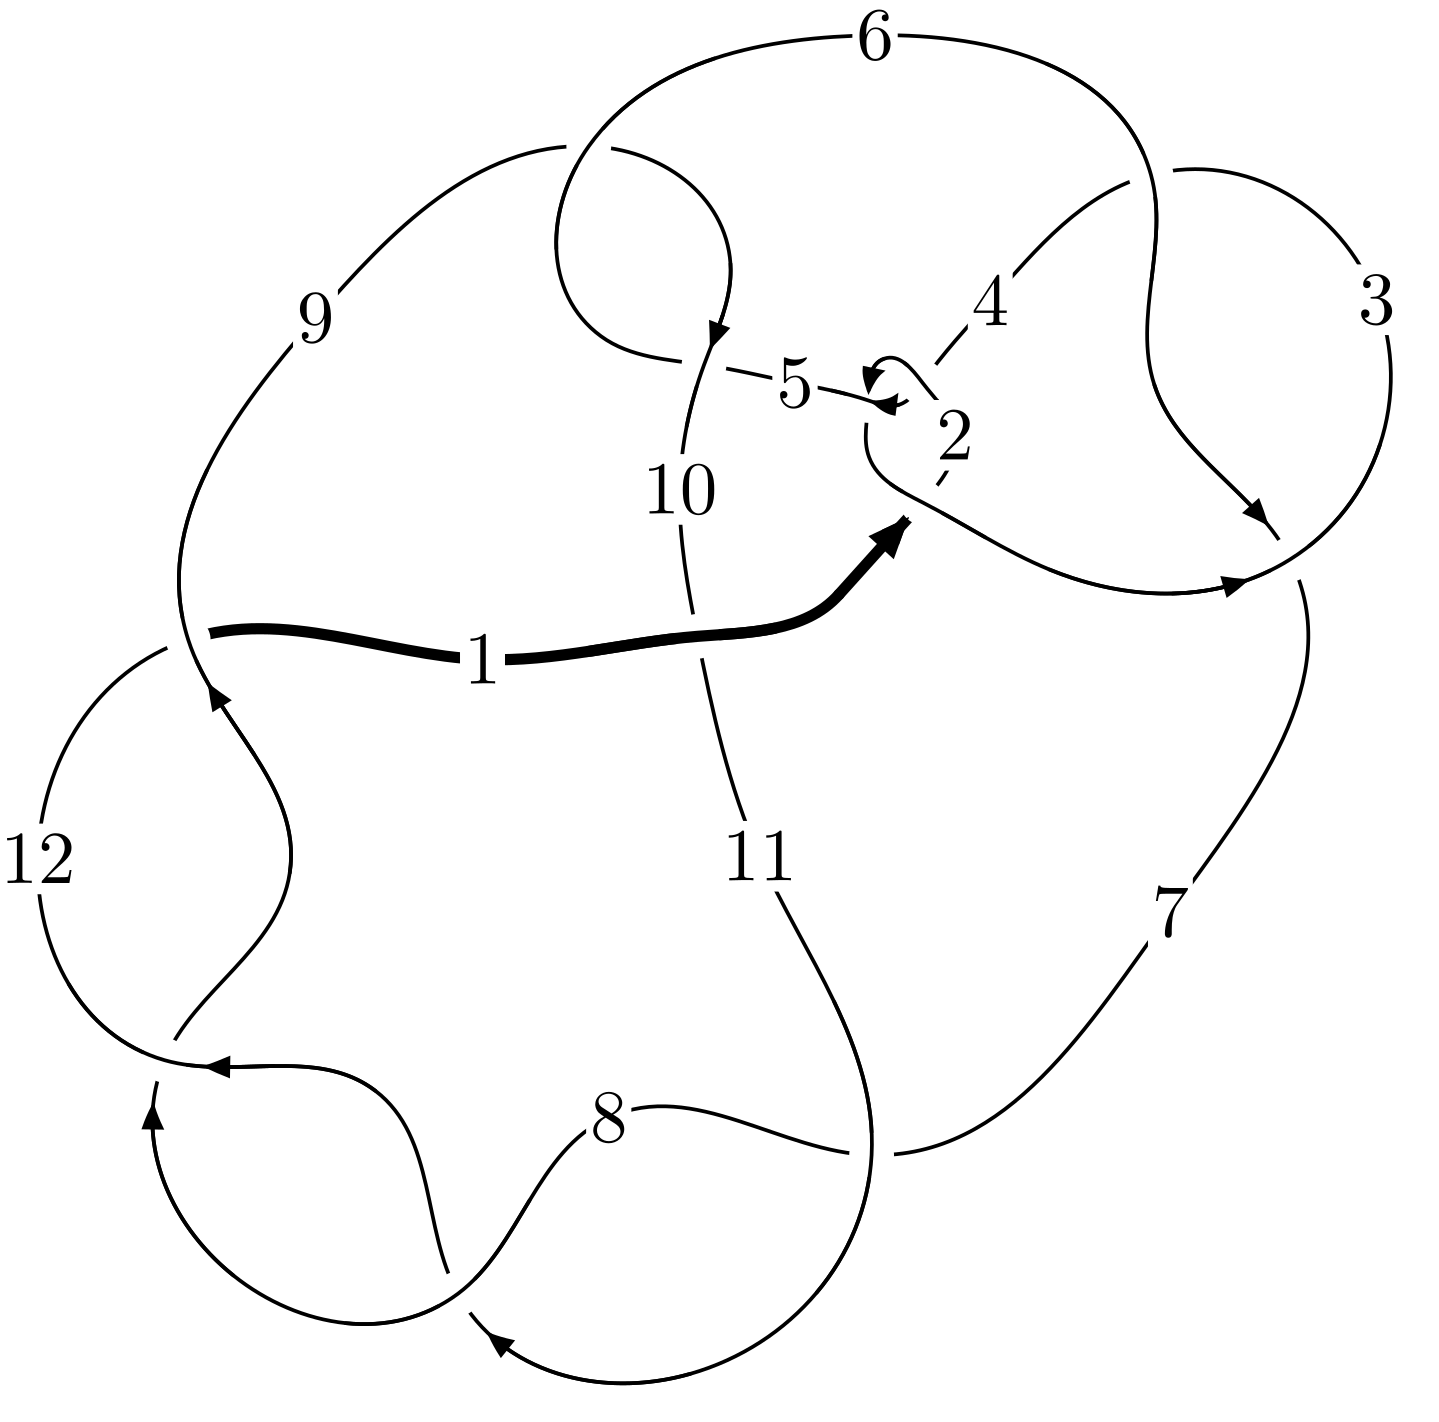
\includegraphics[width=112pt]{../../../GIT/diagram.site/Diagrams/png/2193_12n_0104.png}\\
\ \ \ A knot diagram\footnotemark}&
\allowdisplaybreaks
\textbf{Linearized knot diagam} \\
\cline{2-2}
 &
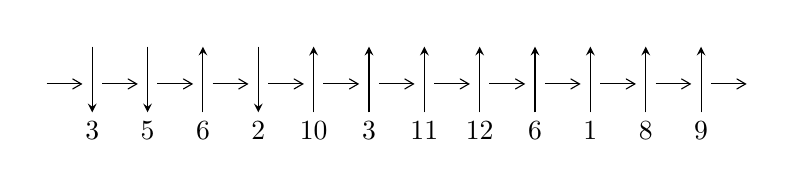
\begin{tikzpicture}[x=20pt, y=17pt]
	% nodes
	\node (C0) at (0, 0) {};
	\node (C1) at (1, 0) {};
	\node (C1U) at (1, +1) {};
	\node (C1D) at (1, -1) {3};

	\node (C2) at (2, 0) {};
	\node (C2U) at (2, +1) {};
	\node (C2D) at (2, -1) {5};

	\node (C3) at (3, 0) {};
	\node (C3U) at (3, +1) {};
	\node (C3D) at (3, -1) {6};

	\node (C4) at (4, 0) {};
	\node (C4U) at (4, +1) {};
	\node (C4D) at (4, -1) {2};

	\node (C5) at (5, 0) {};
	\node (C5U) at (5, +1) {};
	\node (C5D) at (5, -1) {10};

	\node (C6) at (6, 0) {};
	\node (C6U) at (6, +1) {};
	\node (C6D) at (6, -1) {3};

	\node (C7) at (7, 0) {};
	\node (C7U) at (7, +1) {};
	\node (C7D) at (7, -1) {11};

	\node (C8) at (8, 0) {};
	\node (C8U) at (8, +1) {};
	\node (C8D) at (8, -1) {12};

	\node (C9) at (9, 0) {};
	\node (C9U) at (9, +1) {};
	\node (C9D) at (9, -1) {6};

	\node (C10) at (10, 0) {};
	\node (C10U) at (10, +1) {};
	\node (C10D) at (10, -1) {1};

	\node (C11) at (11, 0) {};
	\node (C11U) at (11, +1) {};
	\node (C11D) at (11, -1) {8};

	\node (C12) at (12, 0) {};
	\node (C12U) at (12, +1) {};
	\node (C12D) at (12, -1) {9};
	\node (C13) at (13, 0) {};

	% arrows
	\draw[->,>={angle 60}]
	(C0) edge (C1) (C1) edge (C2) (C2) edge (C3) (C3) edge (C4) (C4) edge (C5) (C5) edge (C6) (C6) edge (C7) (C7) edge (C8) (C8) edge (C9) (C9) edge (C10) (C10) edge (C11) (C11) edge (C12) (C12) edge (C13) ;	\draw[->,>=stealth]
	(C1U) edge (C1D) (C2U) edge (C2D) (C3D) edge (C3U) (C4U) edge (C4D) (C5D) edge (C5U) (C6D) edge (C6U) (C7D) edge (C7U) (C8D) edge (C8U) (C9D) edge (C9U) (C10D) edge (C10U) (C11D) edge (C11U) (C12D) edge (C12U) ;
	\end{tikzpicture} \\
\hhline{~~} \\& 
\textbf{Solving Sequence} \\ \cline{2-2} 
 &
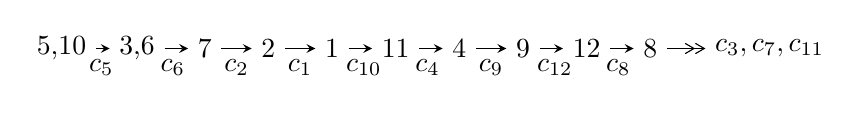
\begin{tikzpicture}[x=23pt, y=7pt]
	% node
	\node (A0) at (-1/8, 0) {5,10};
	\node (A1) at (17/16, 0) {3,6};
	\node (A2) at (17/8, 0) {7};
	\node (A3) at (25/8, 0) {2};
	\node (A4) at (33/8, 0) {1};
	\node (A5) at (41/8, 0) {11};
	\node (A6) at (49/8, 0) {4};
	\node (A7) at (57/8, 0) {9};
	\node (A8) at (65/8, 0) {12};
	\node (A9) at (73/8, 0) {8};
	\node (C1) at (1/2, -1) {$c_{5}$};
	\node (C2) at (13/8, -1) {$c_{6}$};
	\node (C3) at (21/8, -1) {$c_{2}$};
	\node (C4) at (29/8, -1) {$c_{1}$};
	\node (C5) at (37/8, -1) {$c_{10}$};
	\node (C6) at (45/8, -1) {$c_{4}$};
	\node (C7) at (53/8, -1) {$c_{9}$};
	\node (C8) at (61/8, -1) {$c_{12}$};
	\node (C9) at (69/8, -1) {$c_{8}$};
	\node (A10) at (11, 0) {$c_{3},c_{7},c_{11}$};

	% edge
	\draw[->,>=stealth]	
	(A0) edge (A1) (A1) edge (A2) (A2) edge (A3) (A3) edge (A4) (A4) edge (A5) (A5) edge (A6) (A6) edge (A7) (A7) edge (A8) (A8) edge (A9) ;
	\draw[->>,>={angle 60}]	
	(A9) edge (A10);
\end{tikzpicture} \\ 

\end{tabular} \\

\footnotetext{
The image of knot diagram is generated by the software ``\textbf{Draw programme}" developed by Andrew Bartholomew(\url{http://www.layer8.co.uk/maths/draw/index.htm\#Running-draw}), where we modified some parts for our purpose(\url{https://github.com/CATsTAILs/LinksPainter}).
}\phantom \\ \newline 
\centering \textbf{Ideals for irreducible components\footnotemark of $X_{\text{par}}$} 
 
\begin{align*}
I^u_{1}&=\langle 
-3.59372\times10^{41} u^{41}-5.66142\times10^{41} u^{40}+\cdots+7.73697\times10^{41} b-8.41893\times10^{39},\\
\phantom{I^u_{1}}&\phantom{= \langle  }1.32363\times10^{42} u^{41}+2.48624\times10^{42} u^{40}+\cdots+7.73697\times10^{41} a+6.53537\times10^{40},\;u^{42}+2 u^{41}+\cdots+u+1\rangle \\
I^u_{2}&=\langle 
b+1,\;u^5-2 u^4+4 u^3-5 u^2+a+4 u-3,\;u^6- u^5+3 u^4-2 u^3+2 u^2- u-1\rangle \\
\\
\end{align*}
\raggedright * 2 irreducible components of $\dim_{\mathbb{C}}=0$, with total 48 representations.\\
\footnotetext{All coefficients of polynomials are rational numbers. But the coefficients are sometimes approximated in decimal forms when there is not enough margin.}
\newpage
\renewcommand{\arraystretch}{1}
\centering \section*{I. $I^u_{1}= \langle -3.59\times10^{41} u^{41}-5.66\times10^{41} u^{40}+\cdots+7.74\times10^{41} b-8.42\times10^{39},\;1.32\times10^{42} u^{41}+2.49\times10^{42} u^{40}+\cdots+7.74\times10^{41} a+6.54\times10^{40},\;u^{42}+2 u^{41}+\cdots+u+1 \rangle$}
\flushleft \textbf{(i) Arc colorings}\\
\begin{tabular}{m{7pt} m{180pt} m{7pt} m{180pt} }
\flushright $a_{5}=$&$\begin{pmatrix}1\\0\end{pmatrix}$ \\
\flushright $a_{10}=$&$\begin{pmatrix}0\\u\end{pmatrix}$ \\
\flushright $a_{3}=$&$\begin{pmatrix}-1.71079 u^{41}-3.21345 u^{40}+\cdots+10.5415 u-0.0844693\\0.464486 u^{41}+0.731736 u^{40}+\cdots-1.23542 u+0.0108814\end{pmatrix}$ \\
\flushright $a_{6}=$&$\begin{pmatrix}1\\- u^2\end{pmatrix}$ \\
\flushright $a_{7}=$&$\begin{pmatrix}1.20935 u^{41}+1.90913 u^{40}+\cdots-3.32862 u+1.65557\\-0.182245 u^{41}-0.291497 u^{40}+\cdots+0.535851 u-0.403264\end{pmatrix}$ \\
\flushright $a_{2}=$&$\begin{pmatrix}-1.24630 u^{41}-2.48172 u^{40}+\cdots+9.30604 u-0.0735879\\0.464486 u^{41}+0.731736 u^{40}+\cdots-1.23542 u+0.0108814\end{pmatrix}$ \\
\flushright $a_{1}=$&$\begin{pmatrix}1.24139 u^{41}+1.95441 u^{40}+\cdots-3.49255 u+1.76187\\-0.0320409 u^{41}-0.0452803 u^{40}+\cdots+0.163934 u-0.106300\end{pmatrix}$ \\
\flushright $a_{11}=$&$\begin{pmatrix}0.722940 u^{41}+1.09186 u^{40}+\cdots-1.22903 u+1.55759\\-0.0729864 u^{41}-0.0536384 u^{40}+\cdots+1.18829 u-0.138312\end{pmatrix}$ \\
\flushright $a_{4}=$&$\begin{pmatrix}-1.79877 u^{41}-3.35612 u^{40}+\cdots+10.8087 u-0.281705\\0.474629 u^{41}+0.743231 u^{40}+\cdots-1.29010 u+0.0441881\end{pmatrix}$ \\
\flushright $a_{9}=$&$\begin{pmatrix}- u\\u^3+u\end{pmatrix}$ \\
\flushright $a_{12}=$&$\begin{pmatrix}0.986423 u^{41}+1.55821 u^{40}+\cdots-2.67406 u+1.14887\\0.258550 u^{41}+0.408387 u^{40}+\cdots-0.795796 u+0.620421\end{pmatrix}$ \\
\flushright $a_{8}=$&$\begin{pmatrix}-0.549074 u^{41}-0.889586 u^{40}+\cdots+0.0457032 u-1.27204\\-0.183879 u^{41}-0.191517 u^{40}+\cdots+1.29243 u-0.478058\end{pmatrix}$\\&\end{tabular}
\flushleft \textbf{(ii) Obstruction class $= -1$}\\~\\
\flushleft \textbf{(iii) Cusp Shapes $= -7.55767 u^{41}-15.9158 u^{40}+\cdots+73.6479 u+19.0106$}\\~\\
\newpage\renewcommand{\arraystretch}{1}
\flushleft \textbf{(iv) u-Polynomials at the component}\newline \\
\begin{tabular}{m{50pt}|m{274pt}}
Crossings & \hspace{64pt}u-Polynomials at each crossing \\
\hline $$\begin{aligned}c_{1}\end{aligned}$$&$\begin{aligned}
&u^{42}+13 u^{41}+\cdots+804 u+1
\end{aligned}$\\
\hline $$\begin{aligned}c_{2},c_{4}\end{aligned}$$&$\begin{aligned}
&u^{42}-7 u^{41}+\cdots-32 u+1
\end{aligned}$\\
\hline $$\begin{aligned}c_{3},c_{6}\end{aligned}$$&$\begin{aligned}
&u^{42}+5 u^{41}+\cdots-256 u+64
\end{aligned}$\\
\hline $$\begin{aligned}c_{5},c_{9}\end{aligned}$$&$\begin{aligned}
&u^{42}-2 u^{41}+\cdots- u+1
\end{aligned}$\\
\hline $$\begin{aligned}c_{7},c_{8},c_{11}\\c_{12}\end{aligned}$$&$\begin{aligned}
&u^{42}-2 u^{41}+\cdots+u+1
\end{aligned}$\\
\hline $$\begin{aligned}c_{10}\end{aligned}$$&$\begin{aligned}
&u^{42}+14 u^{41}+\cdots+5149 u+1583
\end{aligned}$\\
\hline
\end{tabular}\\~\\
\newpage\renewcommand{\arraystretch}{1}
\flushleft \textbf{(v) Riley Polynomials at the component}\newline \\
\begin{tabular}{m{50pt}|m{274pt}}
Crossings & \hspace{64pt}Riley Polynomials at each crossing \\
\hline $$\begin{aligned}c_{1}\end{aligned}$$&$\begin{aligned}
&y^{42}+39 y^{41}+\cdots-608644 y+1
\end{aligned}$\\
\hline $$\begin{aligned}c_{2},c_{4}\end{aligned}$$&$\begin{aligned}
&y^{42}-13 y^{41}+\cdots-804 y+1
\end{aligned}$\\
\hline $$\begin{aligned}c_{3},c_{6}\end{aligned}$$&$\begin{aligned}
&y^{42}-39 y^{41}+\cdots-253952 y+4096
\end{aligned}$\\
\hline $$\begin{aligned}c_{5},c_{9}\end{aligned}$$&$\begin{aligned}
&y^{42}+10 y^{41}+\cdots-7 y+1
\end{aligned}$\\
\hline $$\begin{aligned}c_{7},c_{8},c_{11}\\c_{12}\end{aligned}$$&$\begin{aligned}
&y^{42}-50 y^{41}+\cdots-7 y+1
\end{aligned}$\\
\hline $$\begin{aligned}c_{10}\end{aligned}$$&$\begin{aligned}
&y^{42}-26 y^{41}+\cdots-65134235 y+2505889
\end{aligned}$\\
\hline
\end{tabular}\\~\\
\newpage\flushleft \textbf{(vi) Complex Volumes and Cusp Shapes}
$$\begin{array}{c|c|c}  
\text{Solutions to }I^u_{1}& \I (\text{vol} + \sqrt{-1}CS) & \text{Cusp shape}\\
 \hline 
\begin{aligned}
u &= \phantom{-}1.01452\phantom{ +0.000000I} \\
a &= \phantom{-}0.159707\phantom{ +0.000000I} \\
b &= \phantom{-}0.426201\phantom{ +0.000000I}\end{aligned}
 & \phantom{-}7.18041\phantom{ +0.000000I} & \phantom{-}14.5060\phantom{ +0.000000I} \\ \hline\begin{aligned}
u &= \phantom{-}0.501113 + 0.767004 I \\
a &= \phantom{-}0.191771 - 1.283310 I \\
b &= -0.669285 + 1.060730 I\end{aligned}
 & \phantom{-}7.44472 + 4.92121 I & \phantom{-}8.52470 - 6.69865 I \\ \hline\begin{aligned}
u &= \phantom{-}0.501113 - 0.767004 I \\
a &= \phantom{-}0.191771 + 1.283310 I \\
b &= -0.669285 - 1.060730 I\end{aligned}
 & \phantom{-}7.44472 - 4.92121 I & \phantom{-}8.52470 + 6.69865 I \\ \hline\begin{aligned}
u &= -0.453853 + 0.695369 I \\
a &= \phantom{-}0.247010 + 1.284860 I \\
b &= -0.719295 - 0.792687 I\end{aligned}
 & -0.28964 - 3.57536 I & \phantom{-}6.37219 + 9.69003 I \\ \hline\begin{aligned}
u &= -0.453853 - 0.695369 I \\
a &= \phantom{-}0.247010 - 1.284860 I \\
b &= -0.719295 + 0.792687 I\end{aligned}
 & -0.28964 + 3.57536 I & \phantom{-}6.37219 - 9.69003 I \\ \hline\begin{aligned}
u &= -0.161979 + 0.776395 I \\
a &= \phantom{-}0.051090 + 0.752460 I \\
b &= -1.48780 - 0.42283 I\end{aligned}
 & \phantom{-}4.30541 - 1.84849 I & \phantom{-}3.64107 + 3.02333 I \\ \hline\begin{aligned}
u &= -0.161979 - 0.776395 I \\
a &= \phantom{-}0.051090 - 0.752460 I \\
b &= -1.48780 + 0.42283 I\end{aligned}
 & \phantom{-}4.30541 + 1.84849 I & \phantom{-}3.64107 - 3.02333 I \\ \hline\begin{aligned}
u &= \phantom{-}0.912511 + 0.794551 I \\
a &= -0.419329 - 0.751716 I \\
b &= \phantom{-}0.631065 + 1.077450 I\end{aligned}
 & \phantom{-}6.12642 + 3.75190 I & \phantom{-}10.63580 - 4.55895 I \\ \hline\begin{aligned}
u &= \phantom{-}0.912511 - 0.794551 I \\
a &= -0.419329 + 0.751716 I \\
b &= \phantom{-}0.631065 - 1.077450 I\end{aligned}
 & \phantom{-}6.12642 - 3.75190 I & \phantom{-}10.63580 + 4.55895 I \\ \hline\begin{aligned}
u &= -0.891381 + 0.841839 I \\
a &= -0.506949 + 0.850686 I \\
b &= \phantom{-}0.658034 - 1.240570 I\end{aligned}
 & \phantom{-}14.7689 - 5.7297 I & \phantom{-}11.79655 + 3.54668 I\\
 \hline 
 \end{array}$$\newpage$$\begin{array}{c|c|c}  
\text{Solutions to }I^u_{1}& \I (\text{vol} + \sqrt{-1}CS) & \text{Cusp shape}\\
 \hline 
\begin{aligned}
u &= -0.891381 - 0.841839 I \\
a &= -0.506949 - 0.850686 I \\
b &= \phantom{-}0.658034 + 1.240570 I\end{aligned}
 & \phantom{-}14.7689 + 5.7297 I & \phantom{-}11.79655 - 3.54668 I \\ \hline\begin{aligned}
u &= -0.985080 + 0.753794 I \\
a &= -0.386102 + 0.573806 I \\
b &= \phantom{-}0.715924 - 0.874389 I\end{aligned}
 & \phantom{-}3.30789 - 0.29459 I & \phantom{-}6.00000 + 0. I\phantom{ +0.000000I} \\ \hline\begin{aligned}
u &= -0.985080 - 0.753794 I \\
a &= -0.386102 - 0.573806 I \\
b &= \phantom{-}0.715924 + 0.874389 I\end{aligned}
 & \phantom{-}3.30789 + 0.29459 I & \phantom{-}6.00000 + 0. I\phantom{ +0.000000I} \\ \hline\begin{aligned}
u &= -0.803175 + 1.000510 I \\
a &= \phantom{-}0.83087 - 1.30330 I \\
b &= \phantom{-}0.831506 + 0.932621 I\end{aligned}
 & \phantom{-}14.2431 - 0.5975 I & \phantom{-}11.31138 + 0. I\phantom{ +0.000000I} \\ \hline\begin{aligned}
u &= -0.803175 - 1.000510 I \\
a &= \phantom{-}0.83087 + 1.30330 I \\
b &= \phantom{-}0.831506 - 0.932621 I\end{aligned}
 & \phantom{-}14.2431 + 0.5975 I & \phantom{-}11.31138 + 0. I\phantom{ +0.000000I} \\ \hline\begin{aligned}
u &= \phantom{-}0.538055 + 0.454086 I \\
a &= \phantom{-}2.48988 - 0.58955 I \\
b &= -0.551064 - 0.378134 I\end{aligned}
 & \phantom{-}8.24921 - 1.23307 I & \phantom{-}10.61321 - 2.35997 I \\ \hline\begin{aligned}
u &= \phantom{-}0.538055 - 0.454086 I \\
a &= \phantom{-}2.48988 + 0.58955 I \\
b &= -0.551064 + 0.378134 I\end{aligned}
 & \phantom{-}8.24921 + 1.23307 I & \phantom{-}10.61321 + 2.35997 I \\ \hline\begin{aligned}
u &= \phantom{-}0.347293 + 0.590519 I \\
a &= \phantom{-}0.19395 - 1.58608 I \\
b &= -0.859706 + 0.416440 I\end{aligned}
 & -1.72808 + 1.17860 I & -0.84051 - 1.97476 I \\ \hline\begin{aligned}
u &= \phantom{-}0.347293 - 0.590519 I \\
a &= \phantom{-}0.19395 + 1.58608 I \\
b &= -0.859706 - 0.416440 I\end{aligned}
 & -1.72808 - 1.17860 I & -0.84051 + 1.97476 I \\ \hline\begin{aligned}
u &= \phantom{-}1.043690 + 0.800779 I \\
a &= -0.495482 - 0.469030 I \\
b &= \phantom{-}0.892411 + 0.841271 I\end{aligned}
 & \phantom{-}5.39547 - 3.53826 I & \phantom{-0.000000 } 0\\
 \hline 
 \end{array}$$\newpage$$\begin{array}{c|c|c}  
\text{Solutions to }I^u_{1}& \I (\text{vol} + \sqrt{-1}CS) & \text{Cusp shape}\\
 \hline 
\begin{aligned}
u &= \phantom{-}1.043690 - 0.800779 I \\
a &= -0.495482 + 0.469030 I \\
b &= \phantom{-}0.892411 - 0.841271 I\end{aligned}
 & \phantom{-}5.39547 + 3.53826 I & \phantom{-0.000000 } 0 \\ \hline\begin{aligned}
u &= \phantom{-}0.087517 + 0.669029 I \\
a &= -0.577668 - 0.564351 I \\
b &= -1.323170 + 0.163226 I\end{aligned}
 & -2.60028 + 1.10335 I & \phantom{-}0.72944 - 5.14975 I \\ \hline\begin{aligned}
u &= \phantom{-}0.087517 - 0.669029 I \\
a &= -0.577668 + 0.564351 I \\
b &= -1.323170 - 0.163226 I\end{aligned}
 & -2.60028 - 1.10335 I & \phantom{-}0.72944 + 5.14975 I \\ \hline\begin{aligned}
u &= \phantom{-}0.807134 + 1.059990 I \\
a &= \phantom{-}0.655895 + 1.196400 I \\
b &= \phantom{-}0.925887 - 0.815812 I\end{aligned}
 & \phantom{-}5.27984 + 2.65601 I & \phantom{-0.000000 } 0 \\ \hline\begin{aligned}
u &= \phantom{-}0.807134 - 1.059990 I \\
a &= \phantom{-}0.655895 - 1.196400 I \\
b &= \phantom{-}0.925887 + 0.815812 I\end{aligned}
 & \phantom{-}5.27984 - 2.65601 I & \phantom{-0.000000 } 0 \\ \hline\begin{aligned}
u &= -0.118669 + 1.352730 I \\
a &= \phantom{-}0.692604 - 0.095605 I \\
b &= \phantom{-}0.673600 + 0.068678 I\end{aligned}
 & -3.90139 - 2.12133 I & \phantom{-0.000000 } 0 \\ \hline\begin{aligned}
u &= -0.118669 - 1.352730 I \\
a &= \phantom{-}0.692604 + 0.095605 I \\
b &= \phantom{-}0.673600 - 0.068678 I\end{aligned}
 & -3.90139 + 2.12133 I & \phantom{-0.000000 } 0 \\ \hline\begin{aligned}
u &= -1.061870 + 0.848054 I \\
a &= -0.596141 + 0.421898 I \\
b &= \phantom{-}1.020730 - 0.858173 I\end{aligned}
 & \phantom{-}13.6503 + 6.0084 I & \phantom{-0.000000 } 0 \\ \hline\begin{aligned}
u &= -1.061870 - 0.848054 I \\
a &= -0.596141 - 0.421898 I \\
b &= \phantom{-}1.020730 + 0.858173 I\end{aligned}
 & \phantom{-}13.6503 - 6.0084 I & \phantom{-0.000000 } 0 \\ \hline\begin{aligned}
u &= -0.453110 + 0.434147 I \\
a &= \phantom{-}1.81325 + 1.42213 I \\
b &= -0.588284 + 0.063513 I\end{aligned}
 & \phantom{-}0.308257 + 0.438585 I & \phantom{-}7.79318 - 0.39703 I\\
 \hline 
 \end{array}$$\newpage$$\begin{array}{c|c|c}  
\text{Solutions to }I^u_{1}& \I (\text{vol} + \sqrt{-1}CS) & \text{Cusp shape}\\
 \hline 
\begin{aligned}
u &= -0.453110 - 0.434147 I \\
a &= \phantom{-}1.81325 - 1.42213 I \\
b &= -0.588284 - 0.063513 I\end{aligned}
 & \phantom{-}0.308257 - 0.438585 I & \phantom{-}7.79318 + 0.39703 I \\ \hline\begin{aligned}
u &= -0.851980 + 1.097830 I \\
a &= \phantom{-}0.462368 - 1.207420 I \\
b &= \phantom{-}1.062440 + 0.773956 I\end{aligned}
 & \phantom{-}2.23629 - 6.46162 I & \phantom{-0.000000 } 0 \\ \hline\begin{aligned}
u &= -0.851980 - 1.097830 I \\
a &= \phantom{-}0.462368 + 1.207420 I \\
b &= \phantom{-}1.062440 - 0.773956 I\end{aligned}
 & \phantom{-}2.23629 + 6.46162 I & \phantom{-0.000000 } 0 \\ \hline\begin{aligned}
u &= \phantom{-}0.890810 + 1.092080 I \\
a &= \phantom{-}0.358382 + 1.303470 I \\
b &= \phantom{-}1.16024 - 0.81354 I\end{aligned}
 & \phantom{-}4.46235 + 10.57810 I & \phantom{-0.000000 } 0 \\ \hline\begin{aligned}
u &= \phantom{-}0.890810 - 1.092080 I \\
a &= \phantom{-}0.358382 - 1.303470 I \\
b &= \phantom{-}1.16024 + 0.81354 I\end{aligned}
 & \phantom{-}4.46235 - 10.57810 I & \phantom{-0.000000 } 0 \\ \hline\begin{aligned}
u &= \phantom{-}0.369530 + 1.364470 I \\
a &= \phantom{-}0.633928 + 0.303473 I \\
b &= \phantom{-}0.736491 - 0.206857 I\end{aligned}
 & \phantom{-}2.62006 + 5.04142 I & \phantom{-0.000000 } 0 \\ \hline\begin{aligned}
u &= \phantom{-}0.369530 - 1.364470 I \\
a &= \phantom{-}0.633928 - 0.303473 I \\
b &= \phantom{-}0.736491 + 0.206857 I\end{aligned}
 & \phantom{-}2.62006 - 5.04142 I & \phantom{-0.000000 } 0 \\ \hline\begin{aligned}
u &= -0.91555 + 1.08098 I \\
a &= \phantom{-}0.29416 - 1.39483 I \\
b &= \phantom{-}1.22988 + 0.86093 I\end{aligned}
 & \phantom{-}12.8768 - 13.1889 I & \phantom{-0.000000 } 0 \\ \hline\begin{aligned}
u &= -0.91555 - 1.08098 I \\
a &= \phantom{-}0.29416 + 1.39483 I \\
b &= \phantom{-}1.22988 - 0.86093 I\end{aligned}
 & \phantom{-}12.8768 + 13.1889 I & \phantom{-0.000000 } 0 \\ \hline\begin{aligned}
u &= -0.500346\phantom{ +0.000000I} \\
a &= \phantom{-}6.58730\phantom{ +0.000000I} \\
b &= -1.11870\phantom{ +0.000000I}\end{aligned}
 & \phantom{-}6.69758\phantom{ +0.000000I} & \phantom{-}29.8650\phantom{ +0.000000I}\\
 \hline 
 \end{array}$$\newpage$$\begin{array}{c|c|c}  
\text{Solutions to }I^u_{1}& \I (\text{vol} + \sqrt{-1}CS) & \text{Cusp shape}\\
 \hline 
\begin{aligned}
u &= -0.442850\phantom{ +0.000000I} \\
a &= \phantom{-}0.781638\phantom{ +0.000000I} \\
b &= \phantom{-}0.0358028\phantom{ +0.000000I}\end{aligned}
 & \phantom{-}0.706374\phantom{ +0.000000I} & \phantom{-}14.0900\phantom{ +0.000000I} \\ \hline\begin{aligned}
u &= \phantom{-}0.326673\phantom{ +0.000000I} \\
a &= \phantom{-}11.6043\phantom{ +0.000000I} \\
b &= -1.02253\phantom{ +0.000000I}\end{aligned}
 & -0.833901\phantom{ +0.000000I} & \phantom{-}102.450\phantom{ +0.000000I}\\
 \hline 
 \end{array}$$\newpage\newpage\renewcommand{\arraystretch}{1}
\centering \section*{II. $I^u_{2}= \langle b+1,\;u^5-2 u^4+4 u^3-5 u^2+a+4 u-3,\;u^6- u^5+3 u^4-2 u^3+2 u^2- u-1 \rangle$}
\flushleft \textbf{(i) Arc colorings}\\
\begin{tabular}{m{7pt} m{180pt} m{7pt} m{180pt} }
\flushright $a_{5}=$&$\begin{pmatrix}1\\0\end{pmatrix}$ \\
\flushright $a_{10}=$&$\begin{pmatrix}0\\u\end{pmatrix}$ \\
\flushright $a_{3}=$&$\begin{pmatrix}- u^5+2 u^4-4 u^3+5 u^2-4 u+3\\-1\end{pmatrix}$ \\
\flushright $a_{6}=$&$\begin{pmatrix}1\\- u^2\end{pmatrix}$ \\
\flushright $a_{7}=$&$\begin{pmatrix}1\\- u^2\end{pmatrix}$ \\
\flushright $a_{2}=$&$\begin{pmatrix}- u^5+2 u^4-4 u^3+5 u^2-4 u+2\\-1\end{pmatrix}$ \\
\flushright $a_{1}=$&$\begin{pmatrix}-1\\0\end{pmatrix}$ \\
\flushright $a_{11}=$&$\begin{pmatrix}u\\u\end{pmatrix}$ \\
\flushright $a_{4}=$&$\begin{pmatrix}- u^5+2 u^4-4 u^3+5 u^2-4 u+3\\-1\end{pmatrix}$ \\
\flushright $a_{9}=$&$\begin{pmatrix}- u\\u^3+u\end{pmatrix}$ \\
\flushright $a_{12}=$&$\begin{pmatrix}u^4+u^2-1\\- u^5+u^4-2 u^3+u^2- u-1\end{pmatrix}$ \\
\flushright $a_{8}=$&$\begin{pmatrix}- u^4- u^2+1\\- u^4-2 u^2\end{pmatrix}$\\&\end{tabular}
\flushleft \textbf{(ii) Obstruction class $= 1$}\\~\\
\flushleft \textbf{(iii) Cusp Shapes $= 7 u^5-7 u^4+21 u^3-17 u^2+20 u-12$}\\~\\
\newpage\renewcommand{\arraystretch}{1}
\flushleft \textbf{(iv) u-Polynomials at the component}\newline \\
\begin{tabular}{m{50pt}|m{274pt}}
Crossings & \hspace{64pt}u-Polynomials at each crossing \\
\hline $$\begin{aligned}c_{1},c_{2}\end{aligned}$$&$\begin{aligned}
&(u-1)^6
\end{aligned}$\\
\hline $$\begin{aligned}c_{3},c_{6}\end{aligned}$$&$\begin{aligned}
&u^6
\end{aligned}$\\
\hline $$\begin{aligned}c_{4}\end{aligned}$$&$\begin{aligned}
&(u+1)^6
\end{aligned}$\\
\hline $$\begin{aligned}c_{5},c_{10}\end{aligned}$$&$\begin{aligned}
&u^6- u^5+3 u^4-2 u^3+2 u^2- u-1
\end{aligned}$\\
\hline $$\begin{aligned}c_{7},c_{8}\end{aligned}$$&$\begin{aligned}
&u^6+u^5-3 u^4-2 u^3+2 u^2- u-1
\end{aligned}$\\
\hline $$\begin{aligned}c_{9}\end{aligned}$$&$\begin{aligned}
&u^6+u^5+3 u^4+2 u^3+2 u^2+u-1
\end{aligned}$\\
\hline $$\begin{aligned}c_{11},c_{12}\end{aligned}$$&$\begin{aligned}
&u^6- u^5-3 u^4+2 u^3+2 u^2+u-1
\end{aligned}$\\
\hline
\end{tabular}\\~\\
\newpage\renewcommand{\arraystretch}{1}
\flushleft \textbf{(v) Riley Polynomials at the component}\newline \\
\begin{tabular}{m{50pt}|m{274pt}}
Crossings & \hspace{64pt}Riley Polynomials at each crossing \\
\hline $$\begin{aligned}c_{1},c_{2},c_{4}\end{aligned}$$&$\begin{aligned}
&(y-1)^6
\end{aligned}$\\
\hline $$\begin{aligned}c_{3},c_{6}\end{aligned}$$&$\begin{aligned}
&y^6
\end{aligned}$\\
\hline $$\begin{aligned}c_{5},c_{9},c_{10}\end{aligned}$$&$\begin{aligned}
&y^6+5 y^5+9 y^4+4 y^3-6 y^2-5 y+1
\end{aligned}$\\
\hline $$\begin{aligned}c_{7},c_{8},c_{11}\\c_{12}\end{aligned}$$&$\begin{aligned}
&y^6-7 y^5+17 y^4-16 y^3+6 y^2-5 y+1
\end{aligned}$\\
\hline
\end{tabular}\\~\\
\newpage\flushleft \textbf{(vi) Complex Volumes and Cusp Shapes}
$$\begin{array}{c|c|c}  
\text{Solutions to }I^u_{2}& \I (\text{vol} + \sqrt{-1}CS) & \text{Cusp shape}\\
 \hline 
\begin{aligned}
u &= \phantom{-}0.873214\phantom{ +0.000000I} \\
a &= \phantom{-}1.31147\phantom{ +0.000000I} \\
b &= -1.00000\phantom{ +0.000000I}\end{aligned}
 & \phantom{-}6.01515\phantom{ +0.000000I} & \phantom{-}5.96810\phantom{ +0.000000I} \\ \hline\begin{aligned}
u &= -0.138835 + 1.234450 I \\
a &= -0.631845 + 0.143944 I \\
b &= -1.00000\phantom{ +0.000000I}\end{aligned}
 & -4.60518 - 1.97241 I & -1.94905 + 2.83524 I \\ \hline\begin{aligned}
u &= -0.138835 - 1.234450 I \\
a &= -0.631845 - 0.143944 I \\
b &= -1.00000\phantom{ +0.000000I}\end{aligned}
 & -4.60518 + 1.97241 I & -1.94905 - 2.83524 I \\ \hline\begin{aligned}
u &= \phantom{-}0.408802 + 1.276380 I \\
a &= -0.453123 - 0.323434 I \\
b &= -1.00000\phantom{ +0.000000I}\end{aligned}
 & \phantom{-}2.05064 + 4.59213 I & \phantom{-}3.43197 - 0.44648 I \\ \hline\begin{aligned}
u &= \phantom{-}0.408802 - 1.276380 I \\
a &= -0.453123 + 0.323434 I \\
b &= -1.00000\phantom{ +0.000000I}\end{aligned}
 & \phantom{-}2.05064 - 4.59213 I & \phantom{-}3.43197 + 0.44648 I \\ \hline\begin{aligned}
u &= -0.413150\phantom{ +0.000000I} \\
a &= \phantom{-}5.85846\phantom{ +0.000000I} \\
b &= -1.00000\phantom{ +0.000000I}\end{aligned}
 & -0.906083\phantom{ +0.000000I} & -24.9340\phantom{ +0.000000I}\\
 \hline 
 \end{array}$$\newpage
\newpage\renewcommand{\arraystretch}{1}
\centering \section*{ III. u-Polynomials}
\begin{tabular}{m{50pt}|m{274pt}}
Crossings & \hspace{64pt}u-Polynomials at each crossing \\
\hline $$\begin{aligned}c_{1}\end{aligned}$$&$\begin{aligned}
&((u-1)^6)(u^{42}+13 u^{41}+\cdots+804 u+1)
\end{aligned}$\\
\hline $$\begin{aligned}c_{2}\end{aligned}$$&$\begin{aligned}
&((u-1)^6)(u^{42}-7 u^{41}+\cdots-32 u+1)
\end{aligned}$\\
\hline $$\begin{aligned}c_{3},c_{6}\end{aligned}$$&$\begin{aligned}
&u^6(u^{42}+5 u^{41}+\cdots-256 u+64)
\end{aligned}$\\
\hline $$\begin{aligned}c_{4}\end{aligned}$$&$\begin{aligned}
&((u+1)^6)(u^{42}-7 u^{41}+\cdots-32 u+1)
\end{aligned}$\\
\hline $$\begin{aligned}c_{5}\end{aligned}$$&$\begin{aligned}
&(u^6- u^5+3 u^4-2 u^3+2 u^2- u-1)(u^{42}-2 u^{41}+\cdots- u+1)
\end{aligned}$\\
\hline $$\begin{aligned}c_{7},c_{8}\end{aligned}$$&$\begin{aligned}
&(u^6+u^5-3 u^4-2 u^3+2 u^2- u-1)(u^{42}-2 u^{41}+\cdots+u+1)
\end{aligned}$\\
\hline $$\begin{aligned}c_{9}\end{aligned}$$&$\begin{aligned}
&(u^6+u^5+3 u^4+2 u^3+2 u^2+u-1)(u^{42}-2 u^{41}+\cdots- u+1)
\end{aligned}$\\
\hline $$\begin{aligned}c_{10}\end{aligned}$$&$\begin{aligned}
&(u^6- u^5+3 u^4-2 u^3+2 u^2- u-1)(u^{42}+14 u^{41}+\cdots+5149 u+1583)
\end{aligned}$\\
\hline $$\begin{aligned}c_{11},c_{12}\end{aligned}$$&$\begin{aligned}
&(u^6- u^5-3 u^4+2 u^3+2 u^2+u-1)(u^{42}-2 u^{41}+\cdots+u+1)
\end{aligned}$\\
\hline
\end{tabular}\newpage\renewcommand{\arraystretch}{1}
\centering \section*{ IV. Riley Polynomials}
\begin{tabular}{m{50pt}|m{274pt}}
Crossings & \hspace{64pt}Riley Polynomials at each crossing \\
\hline $$\begin{aligned}c_{1}\end{aligned}$$&$\begin{aligned}
&((y-1)^6)(y^{42}+39 y^{41}+\cdots-608644 y+1)
\end{aligned}$\\
\hline $$\begin{aligned}c_{2},c_{4}\end{aligned}$$&$\begin{aligned}
&((y-1)^6)(y^{42}-13 y^{41}+\cdots-804 y+1)
\end{aligned}$\\
\hline $$\begin{aligned}c_{3},c_{6}\end{aligned}$$&$\begin{aligned}
&y^6(y^{42}-39 y^{41}+\cdots-253952 y+4096)
\end{aligned}$\\
\hline $$\begin{aligned}c_{5},c_{9}\end{aligned}$$&$\begin{aligned}
&(y^6+5 y^5+\cdots-5 y+1)(y^{42}+10 y^{41}+\cdots-7 y+1)
\end{aligned}$\\
\hline $$\begin{aligned}c_{7},c_{8},c_{11}\\c_{12}\end{aligned}$$&$\begin{aligned}
&(y^6-7 y^5+\cdots-5 y+1)(y^{42}-50 y^{41}+\cdots-7 y+1)
\end{aligned}$\\
\hline $$\begin{aligned}c_{10}\end{aligned}$$&$\begin{aligned}
&(y^6+5 y^5+9 y^4+4 y^3-6 y^2-5 y+1)\\
&\cdot(y^{42}-26 y^{41}+\cdots-65134235 y+2505889)
\end{aligned}$\\
\hline
\end{tabular}
\vskip 2pc
\end{document}